%----------------------------------------------------------------------------------------
%	PACKAGES AND OTHER DOCUMENT CONFIGURATIONS
%----------------------------------------------------------------------------------------
\documentclass[a4paper,11pt]{article}

%Include Packages
%----------------------------------------------------
\usepackage{../Header/KaTeX_LabReport}
\usepackage{lipsum}
% Note: 
% The input command is equivalent to copy-paste the content of the file
% into the current file.

\renewcommand{\thesection}{\Roman{section}} 
\titleformat{\section}[display]%command shape
    {\Huge}%format
    {
        \newpage
        \setlength\fboxsep{0pt}
        \color{gray} \fontsize{20}{5}\selectfont\chaptername\ \thesection
    }%label
    {0pt}{}{}
\titlespacing*{\section}{0pt}{0pt}{20pt}
\renewcommand{\thesubsection}{\thesection: \Roman{subsection}}
\renewcommand{\thesubsubsection}{\thesubsection. \roman{subsubsection}}
\renewcommand{\thesubsection}{\Roman{subsection}}
\titleformat{\subsection}
    {\bfseries\Large}%format
    {\huge\textnormal{\thesubsection}}%label
    {12pt}{}{}

\usepackage{sectsty}
    \sectionfont{\LARGE}
    \subsectionfont{\large}
    \subsubsectionfont{\large}
    \paragraphfont{\large}
\usepackage{titletoc}
    \titlecontents{}[1em]{\addvspace{1pc}\bfseries}      {\contentslabel{3em}}{}
    {\titlerule*[0.3pc]{.}\contentspage}

\usepackage{tocloft}% http://ctan.org/pkg/tocloft
\setlength\cftsecnumwidth{6em}

\renewcommand{\thesubsubsection}{\thesubsection: \roman{subsubsection}}
\titlespacing{\subsubsection}{0pt}{15pt}{5pt}

%Hyperlink Setting
%----------------------------------------------------
\hypersetup{hidelinks,
	colorlinks=true,
	allcolors=black,
	pdfstartview=Fit,
	breaklinks=true
}

% \includeonly{
%     Experiment_01/Lab1_Main,
%     Experiment_02/Lab2_Main,
%     Experiment_07/Lab7_Main,
% }

\begin{document}
%----------------------------------------------------------------------------------------
%	FRONT MATTER
%----------------------------------------------------------------------------------------
% Cover
\thispagestyle{empty}
\begin{titlepage}
    % Warning Filter
    \WarningFilter[latex]{latexfont}{Some font shapes}
    \WarningFilter[latex]{tex}{Underfull \hbox}
    \ActivateWarningFilters[latex]

	%\hspace{0.05\textheight} % Whitespace between the vertical line and title page text
    \parbox{1\textwidth}{ % Paragraph box for holding the title page text, adjust the width to move the title page left or right on the page
		{\Huge\bfseries EIE420 Assignment II \\[0.15\baselineskip] 
        Gray Scale Histrogram}\\[0.15\baselineskip] % Title
		\rule{1\textwidth}{1pt} % Vertical line
        {\Large\textit{Report of EIE420, Digital Image Processing Assignment}}
        \newline
    }
    \parbox{1\textwidth}{
        \vspace{1\baselineskip}
        \large
        Source Code of this assignment could be found at:\newline
        \url{https://github.com/ZeppelinSCB/EIE420-Digital_Image_Processing}
        \newline
    }
    \vspace{100pt} % Whitespace between the title block and the publisher
    \parbox{1\textwidth}{
        {\large by}\\[1.5\baselineskip]
        {\rule[1pt]{200pt}{1pt}} \\[1.25pt]
        {\huge\textsc{Pengrui K. Tong}
            %\begin{CJK*}{UTF8}{bsmi}\Large (湯鵬睿)\end{CJK*}
            }\\
        {\large{Student No: 1220031811}} \\
        \large from EIE420 D1, \newline
        Faculty of Innovation Engeneering, \newline
        Universidade de Ciência e Tecnologia de Macau
    }
		

    \vspace*{\fill}
		Apr 6, 2025 \newline 
        (Coloane, Macao, SAR)
        \vspace{0.7\baselineskip}\newline
        %
\includegraphics[width = 40mm]{MUIT_BlueGold.png}\newline
        
\includegraphics[width = 40mm]{../Header/MUIT_origin.png}\par
        {\small Cover Design by Karl Tong}\\[0.25pt]
        {\small This report is a part of the result for}
        {\small EIE420~Digital~Image~Processing in U.C.T.M}\\[0.25pt]
        {\small \copyright 2025 Pengrui Tong}
\end{titlepage}
\blankpage

% Table of Contents
\tableofcontents
\blankpage

\section{Problem Statement}
Edge detection is crucial for object boundary identification in computer vision for further analysis. For example, scenarios like auto driving, object detetions, or counting objects in a image. In this experiment, we will implement the gradient operator to detect edges in an image.

\section{Procedure}
The gradient operator is a simple and effective method for edge detection, which calculates the intensity gradient of an image at each pixel location. Pixel with large gradient means the intensity changes rapidly, indicating a potential edge. 
In todays experiment, the gradient operator computes the gradient in both the x and y directions, which can be combined to obtain the overall gradient magnitude, like the following equation:
\begin{equation}
    \begin{aligned}
        \nabla f(x,y) &= Max \{ \delta R, \delta L, \delta D, \delta U\} \\
    \end{aligned}
\end{equation}

\subsection{Design of the Algorithm}
The algorithm is designed to detect edges in an image using the gradient operator. The steps are as follows:
\begin{enumerate}
    \item Image Enlargement (Boundary Handling):
    \begin{enumerate}
        \item Create a zero matrix with a 1-pixel border around the original image.
        \item Place the standardized 8-bit image into the enlarged matrix.
    \end{enumerate}
\item Gradient Computation:
    \begin{enumerate}
        \item Calculate absolute horizontal differences:
            \begin{enumerate}
                \item Right-difference: $ |f(x,y) - f(x+1,y)| $.
                \item Left-difference: $ |f(x,y) - f(x-1,y)| $.
            \end{enumerate}
        \item Calculate absolute vertical differences:
            \begin{enumerate}
                \item Down-difference: $ |f(x,y) - f(x,y+1)| $.
                \item Up-difference: $ |f(x,y) - f(x,y-1)| $.
            \end{enumerate}
    \end{enumerate}

\item Post-Processing:
    \begin{enumerate}
        \item Normalize the combined gradient map (\texttt{mapEdge}) to 8-bit range using \texttt{mat2gray} and \texttt{im2uint8}.
        \item Invert the gradient values by subtracting each pixel from 255 (converting to \texttt{double} for arithmetic).
        \item Re-normalize the inverted map to 8-bit range using \texttt{mat2gray} and \texttt{im2uint8} to produce the final edge map.
    \end{enumerate}
\end{enumerate}

\section{Source Code}
\subsection{Code for Main Function}
\lstset{language = Matlab}
    \begin{lstlisting}[basicstyle=\tiny]
    function [mapEdge, mapEdgeSobel, mapEdgePrewitt] = Lab3_GradientOperator(img)
        % Read the image
        img = imread(img);
        % Convert to grayscale if the image is RGB
        if size(img, 3) == 3
            img = rgb2gray(img);
        end
        
        % Edge detection using gradient operator
        mapEdge = EdgeGradient(img);
        
        % Edge detection using Sobel operator
        mapEdgeSobel = EdgeSobel(img);
        
        % Edge detection using Prewitt operator
        mapEdgePrewitt = EdgePrewitt(img);
    end
\end{lstlisting}

\subsubsection{Code for Edge Detection using Gradient Operator}
\lstset{language = Matlab}
    \begin{lstlisting}[basicstyle=\tiny]
    function mapEdge = EdgeGradient(img)
        % Standardize input image
        imgSize = size(img);
        dimention = length(imgSize);
        if dimention == 3 % Assume RGB image
            imgHSV = rgb2hsv(img);
            img8b = uint8(imgHSV(:,:,3) * 255); % Convert double to uint8
        elseif dimention == 2 % Assume grayscale image
            img8b = uint8(img);
        else
            error('Input must be a three or two dimensional matrix');
        end
        % Enlarge the image to avoid boundary problems
        img8bE = zeros(imgSize(1)+2, imgSize(2)+2, "uint8");
        img8bE(2:end-1, 2:end-1) = img8b;
        
        % |f(x,y)-f(x+1,y)|
        dR = abs(img8bE(2:end-1, 2:end-1) - img8bE(3:end, 2:end-1)); % Right
        % |f(x,y)-f(x-1,y)|
        dL = abs(img8bE(2:end-1, 2:end-1) - img8bE(1:end-2, 2:end-1)); % Left
        % |f(x,y)-f(x,y+1)|
        dD = abs(img8bE(2:end-1, 2:end-1) - img8bE(2:end-1, 3:end)); % Down
        % |f(x,y)-f(x,y-1)|
        dU = abs(img8bE(2:end-1, 2:end-1) - img8bE(2:end-1, 1:end-2)); % Up
    
        mapEdge = max(max(dR, dL), max(dD, dU));
        mapEdge = im2uint8(mat2gray(mapEdge));
        mapEdge = 255-double(mapEdge);
        mapEdge = im2uint8(mat2gray(mapEdge));
    
    end
\end{lstlisting}

\section{Discussion}

\subsection{Sample Program Output}
We tested the program three time with different images. To evlauate the performance of our algorithm, we used the following three images:

\begin{figure}[H]
    \centering
    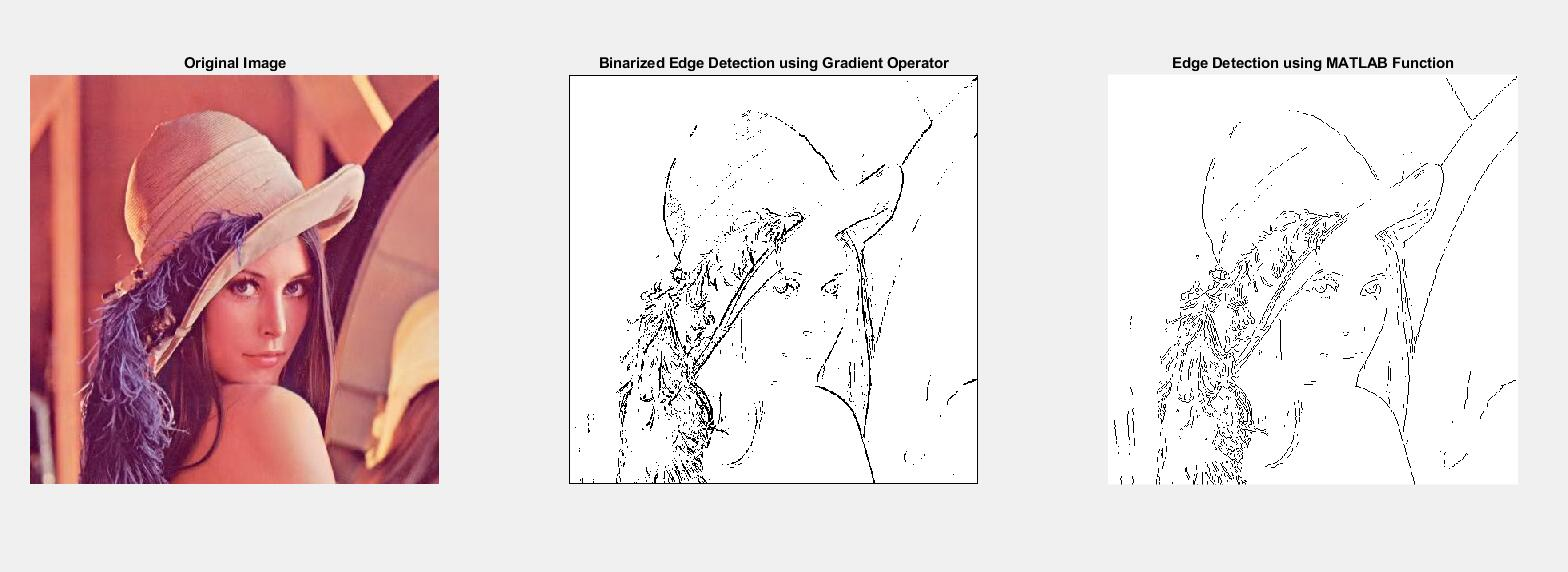
\includegraphics[width=0.8\linewidth]{Demo1.jpg}
    \caption{Lenna}
    \label{pic:Demo_1}
\end{figure}
The first image is the classic "Lenna" image, as shown in figure \ref{pic:Demo_1}. we can see the edges of the image are clearly detected. However, compares to the Matlab function, our code need to manuly adjust the threhold for the binary process, and having difficulty to find the best threshold.

\begin{figure}[H]
    \centering
    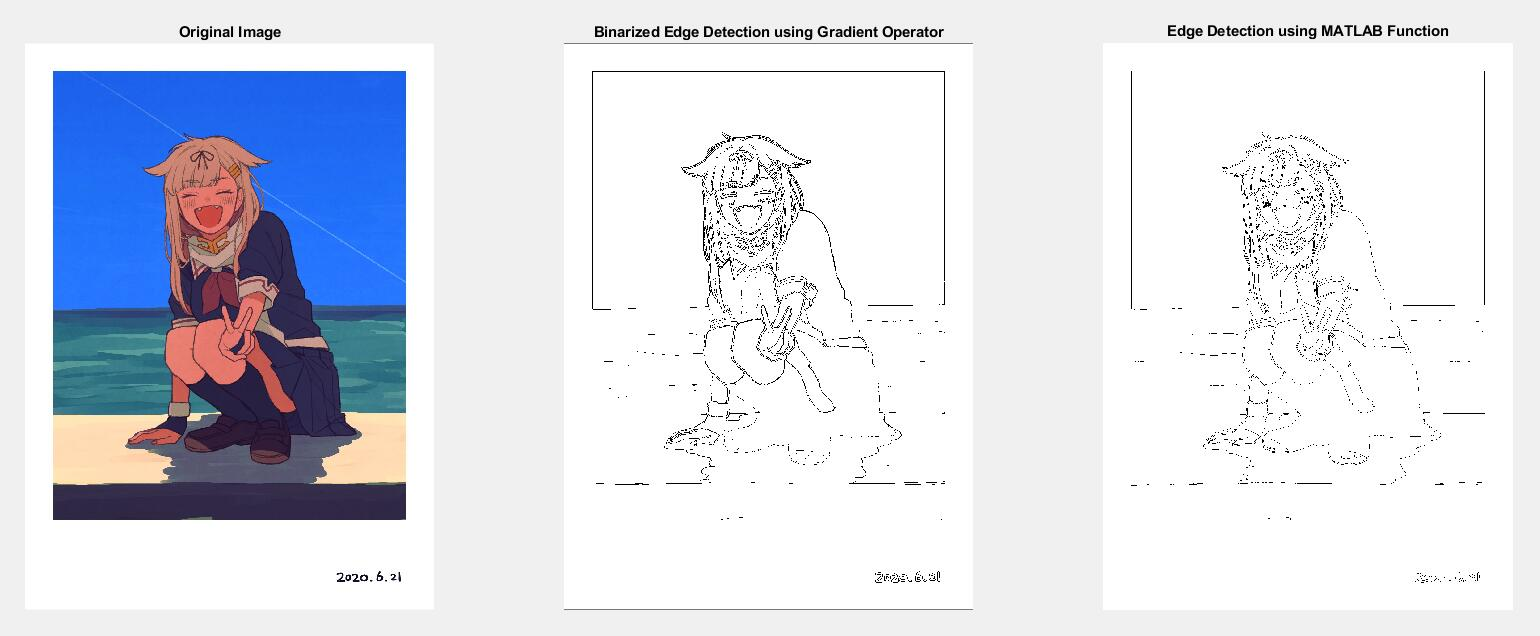
\includegraphics[width=0.8\linewidth]{Demo2.jpg}
    \caption{Comic image}
    \label{pic:Demo_2}
\end{figure}
The second image is a comic image, as shown in figure \ref{pic:Demo_2}. The edges are also clearly detected. And because this image is easier than real photos, our code performs similar to the matlab function.

\begin{figure}[H]
    \centering
    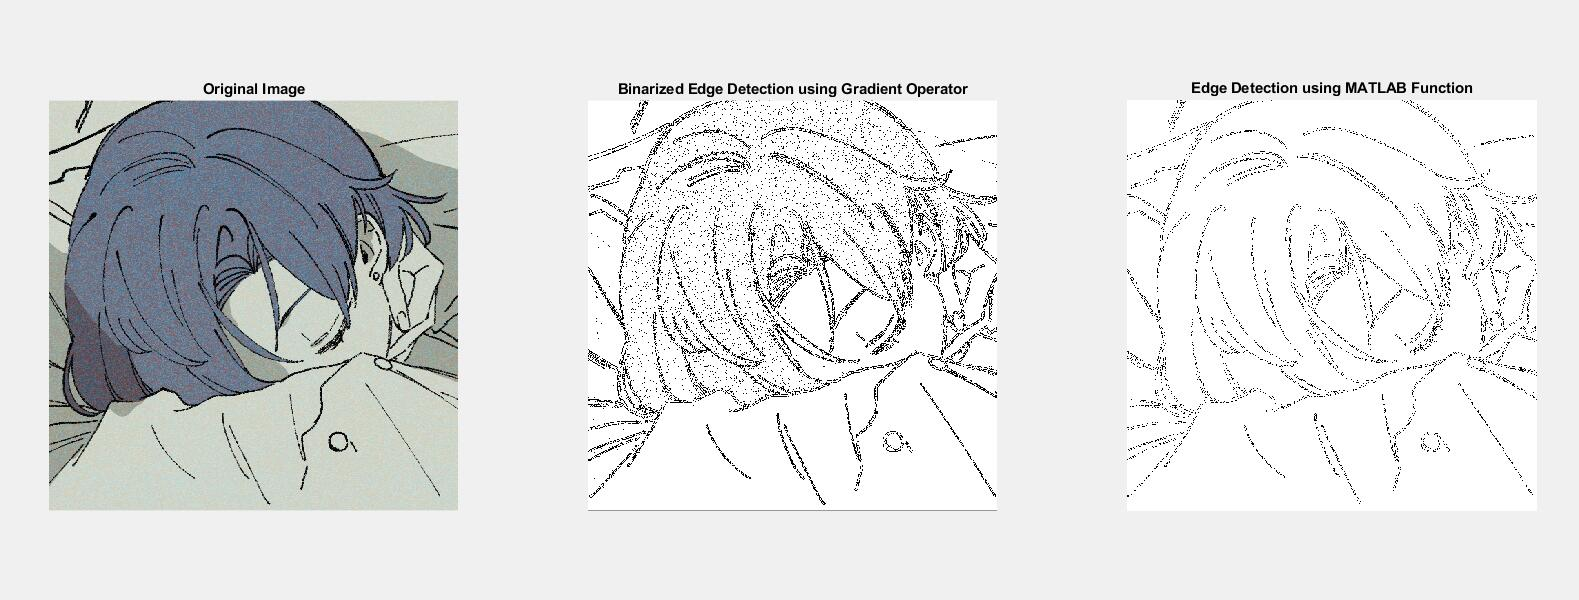
\includegraphics[width=0.8\linewidth]{Demo3-Noise.jpg}
    \caption{Comic image with noise}
    \label{pic:Demo_3}
\end{figure}
The third image is a comic image with added noise, as shown in figure \ref{pic:Demo_3}. Some artist prefer this kind for style for a retro looks. The presence of noise makes edge detection more challenging. While our algorithm is able to detect the edges, the results contains many noise as those are also the pixels with large gradient. Improving the robustness of our algorithm against noise could be a potential area for future work.

\section{Conclusion}
In this experiment, we implemented the gradient operator for edge detection. The algorithm was able to detect edges in various images, including the classic "Lenna" image and a comic image with added noise. However, the algorithm struggled with noise and required manual threshold adjustment for binary processing. Future work could focus on improving robustness against noise and automating threshold selection.

\section{References}
No references were used in this experiment.
\end{document}